% !TEX root = ../main.tex
\chapter{Introduction}
The following experiments explore lasers and their applications as well as interference phenomena.

\section{He-Ne Laser}
The common He-Ne-laser consists of a thin (ca. \SI{1}{\milli\meter} in diameter) glass tube filled with a helium-neon gas mixture.
The gas usually is under a pressure of around \SI{100}{\pascal}, where the partial pressures of helium/neon are dependent of the desired wave length of the laser.
At both ends, resonator mirrors are installed with optional Brewster-windows before them.
These Brewster-windows transmit light only of a specific polarisation direction, other directions are mostly reflected.
This means that a laser with Brewster-windows principally emits linear polarized light (more detailed explanations can be found in \autoref{sec:brewster}).

The functioning can be described as follows:
If a high voltage is applied in the filaments, free electrons are created through gas discharge, which can collide with the helium atoms, moving them into an excited state.
The excited helium atoms can stimulate other neon atoms, inducing a population inversion among them.
The term population inversion refers to a situation in which more electrons are in higher states than others.
This process is called \textbf{optical pumping} and is absolutely obligatory for the functioning of the laser.

Changes of state in the neon atoms emit photons by stimulated emission.
These photons are fed back into the system by the resonator and can stimulate other atoms, effectively amplifying emission of photons.

\section{Brewster-angle}\label{sec:brewster}
\begin{figure}[tb]
	\centering
	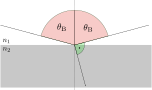
\includegraphics[width=0.6\textwidth]{./img/brewster.pdf}
	\caption[Brewster-angle]{The Brewster-angle}
\end{figure}
When light hits a surface (e.g. glass) it causes dipoles to oscillate inside the material, which radiate and so create reflection and transmission of light.
These dipoles radiate linear polarized light only vertical to their axis of vibration.
If the angle between the reflected and the transmitted light is equal to \SI{90}{\degree}, the intensity of the reflected p-polarized portion disappears, because the dipoles' axis of oscillation is parallel to the direction of transmitted light.
The the s-polarized share, however, is reflected according to Fresnel's law.

By trivial calculations we can show that
\begin{equation}\label{eq:brewster}
	\tan\theta_\text{B}=\frac{n_2}{n_1},
\end{equation}
where $\theta_\text{B}$ denotes the Brewster-angle and $n_2, n_1$ denote the refraction indices of the material and air respectively (assuming the experiment is being condcuted inside of air).

This effect is used inside the He-Ne laser to get a homogenously polarized beam, as only the s-polarized portion of light is reflected by the Brewster-windows, whereas the p-portion can pass them.

\section{Diffraction phenomena}
The following explanations are of minimal extent, as described processes should be familiar by common evidence.

\subsection{Single slit}\label{subsec:single_slit}

\begin{figure}[tb]
	\begin{subfigure}{.51\textwidth}
		\centering
		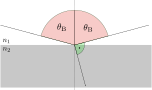
\includegraphics[width=0.6\textwidth]{./img/brewster.pdf}
		\caption[Single slit I]{Path difference deviation}
		\label{fig:path_diff_single}
	\end{subfigure}
	\begin{subfigure}{.51\textwidth}
		\centering
		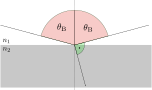
\includegraphics[width=0.6\textwidth]{./img/brewster.pdf}
		\caption[Single slit II]{Angle-distance relation}
		\label{fig:angle_distance_single}
	\end{subfigure}
	\caption[Deviation of single-slit formulae]{Deviation of single-slit formulae}
\end{figure}

Considering \autoref{fig:path_diff_single} we can see that
\begin{equation*}
	\Delta s=b\sin\alpha
\end{equation*}
for the path difference of both beams.

The condition for minima is
\begin{equation}\label{eq:path_diff_min}
	\Delta s = n\cdot\lambda\ ;\qquad n\in\mathbb{N}
\end{equation}
as the transmitted beam is divisible into $2n$ partial beams which cancel out each other in pairs.

The same deliberation can be applied to find the maxima.
It holds
\begin{equation}\label{eq:path_diff_max}
	\Delta s = \left(n+\frac{1}{2}\right)\cdot\lambda\ ;\qquad n\in\mathbb{N}.
\end{equation}
Like this we can divide the beam into $2n+1$ partial beams, the $2n$ beams canceling each other out again, while the last one remains.
This residual beam can be observed as the $n$-th maximum.

Looking at \autoref{fig:angle_distance_single} it holds
\begin{equation}\label{eq:dist_single}
	y_n = d\tan\alpha_n\ ;\qquad n\in\mathbb{N}.
\end{equation}

Assuming the observed angles are small, using equations \ref{eq:path_diff_min}, \ref{eq:path_diff_max} and \ref{eq:dist_single}, we can see that
\begin{equation}\label{eq:single_slit_minima}
	b = \frac{n\lambda d}{y_n} ;\qquad n\in\mathbb{N}.
\end{equation}
for minima and
\begin{equation}\label{eq:single_slit_maxima}
	b = \frac{\left(n+\frac{1}{2}\right)\lambda d}{y_n} ;\qquad n\in\mathbb{N}.
\end{equation}
for maxima of the diffraction pattern.

\subsection{Bridge}
To deduce the diffraction pattern of a bridge, we make use of Babinet's theorem which states that two complementary objects have the same diffraction pattern.
This can be understood considering following thoughts:
Assuming $O$ is the original diffracting object and $\bar{O}$ is its complement viz. that it is opaque where $O$ is transparent and vice versa.
The sum of the amplitudes by the diffractions caused by $O$ and $\bar{O}$ must equal the amplitude of an unobstructed beam.
This means that in places where the light would not have reached without diffraction, the phases of patterns caused by $O$ and $\bar{O}$ must be opposite in phase, effectively causing the amplitude to be negative.
However, for perception of the diffraction patterns not amplitude matters but intensity, which is proportional to the square of the amplitude.

We notice that a bridge of thickness $b$ is the complement of a single-slit of same gap-width, so the diffraction patterns should be the same and we can use the same equations as deviated in \autoref{subsec:single_slit}.

\subsection{Double-slits and lattices}
